\documentclass[12pt]{article}

%packages
%\usepackage{latexsym}
\usepackage{graphicx}
\usepackage{wrapfig}
\usepackage{color}
\usepackage{amsmath}
\usepackage{dsfont}
\usepackage{placeins}
\usepackage{amssymb}
\usepackage{skull}
\usepackage{enumerate}
\usepackage{soul}
\usepackage{alphalph}
\usepackage{hyperref}
\usepackage{enumerate}
\usepackage{listings}
%\usepackage{fancyhdr}

%\fancyhf{} % clear all header and footers
%\renewcommand{\headrulewidth}{0pt} % remove the header rule
%\fancyfoot[LE, LO]{\thepage}


%\usepackage{pstricks,pst-node,pst-tree}

%\usepackage{algpseudocode}
%\usepackage{amsthm}
%\usepackage{hyperref}
%\usepackage{mathrsfs}
%\usepackage{amsfonts}
%\usepackage{bbding}
%\usepackage{listings}
%\usepackage{appendix}
\usepackage[margin=1in]{geometry}
%\geometry{papersize={8.5in,11in},total={6.5in,9in}}
%\usepackage{cancel}
%\usepackage{algorithmic, algorithm}

\definecolor{dkgreen}{rgb}{0,0.6,0}
\definecolor{gray}{rgb}{0.5,0.5,0.5}
\definecolor{mauve}{rgb}{0.58,0,0.82}
\lstset{ %
  language=R,                     % the language of the code
  basicstyle=\footnotesize,       % the size of the fonts that are used for the code
  numbers=left,                   % where to put the line-numbers
  numberstyle=\tiny\color{gray},  % the style that is used for the line-numbers
  stepnumber=1,                   % the step between two line-numbers. If it's 1, each line
                                  % will be numbered
  numbersep=5pt,                  % how far the line-numbers are from the code
  backgroundcolor=\color{white},  % choose the background color. You must add \usepackage{color}
  showspaces=false,               % show spaces adding particular underscores
  showstringspaces=false,         % underline spaces within strings
  showtabs=false,                 % show tabs within strings adding particular underscores
  frame=single,                   % adds a frame around the code
  rulecolor=\color{black},        % if not set, the frame-color may be changed on line-breaks within not-black text (e.g. commens (green here))
  tabsize=2,                      % sets default tabsize to 2 spaces
  captionpos=b,                   % sets the caption-position to bottom
  breaklines=true,                % sets automatic line breaking
  breakatwhitespace=false,        % sets if automatic breaks should only happen at whitespace
  title=\lstname,                 % show the filename of files included with \lstinputlisting;
                                  % also try caption instead of title
  keywordstyle=\color{blue},      % keyword style
  commentstyle=\color{dkgreen},   % comment style
  stringstyle=\color{mauve},      % string literal style
  escapeinside={\%*}{*)},         % if you want to add a comment within your code
  morekeywords={*,...}            % if you want to add more keywords to the set
}

\newcommand{\qu}[1]{``#1''}
\newcommand{\spc}[1]{\\ \vspace{#1cm}}

\newcounter{probnum}
\setcounter{probnum}{1}
\newcounter{numpts}
\setcounter{numpts}{0}

%create definition to allow local margin changes
\def\changemargin#1#2{\list{}{\rightmargin#2\leftmargin#1}\item[]}
\let\endchangemargin=\endlist 

%allow equations to span multiple pages
\allowdisplaybreaks

%define colors and color typesetting conveniences
\definecolor{gray}{rgb}{0.5,0.5,0.5}
\definecolor{black}{rgb}{0,0,0}
\definecolor{white}{rgb}{1,1,1}
\definecolor{blue}{rgb}{0.5,0.5,1}
\newcommand{\inblue}[1]{\color{blue}#1 \color{black}}
\definecolor{green}{rgb}{0.133,0.545,0.133}
\newcommand{\ingreen}[1]{\color{green}#1 \color{black}}
\definecolor{yellow}{rgb}{1,0.549,0}
\newcommand{\inyellow}[1]{\color{yellow}#1 \color{black}}
\definecolor{red}{rgb}{1,0.133,0.133}
\newcommand{\inred}[1]{\color{red}#1 \color{black}}
\definecolor{purple}{rgb}{0.58,0,0.827}
\newcommand{\inpurple}[1]{\color{purple}#1 \color{black}}
\definecolor{gray}{rgb}{0.5,0.5,0.5}
\newcommand{\ingray}[1]{\color{gray}#1 \color{black}}
\definecolor{backgcode}{rgb}{0.97,0.97,0.8}
\definecolor{Brown}{cmyk}{0,0.81,1,0.60}
\definecolor{OliveGreen}{cmyk}{0.64,0,0.95,0.40}
\definecolor{CadetBlue}{cmyk}{0.62,0.57,0.23,0}

%define new math operators
\DeclareMathOperator*{\argmax}{arg\,max~}
\DeclareMathOperator*{\argmin}{arg\,min~}
\DeclareMathOperator*{\argsup}{arg\,sup~}
\DeclareMathOperator*{\arginf}{arg\,inf~}
\DeclareMathOperator*{\convolution}{\text{\Huge{$\ast$}}}
\newcommand{\infconv}[2]{\convolution^\infty_{#1 = 1} #2}
%true functions

%%%% GENERAL SHORTCUTS

\makeatletter
\newalphalph{\alphmult}[mult]{\@alph}{26}
\renewcommand{\labelenumi}{(\alphmult{\value{enumi}})}
\renewcommand{\theenumi}{\AlphAlph{\value{enumi}}}
\makeatother
%shortcuts for pure typesetting conveniences
\newcommand{\bv}[1]{\boldsymbol{#1}}

%shortcuts for compound constants
\newcommand{\BetaDistrConst}{\dfrac{\Gamma(\alpha + \beta)}{\Gamma(\alpha)\Gamma(\beta)}}
\newcommand{\NormDistrConst}{\dfrac{1}{\sqrt{2\pi\sigma^2}}}

%shortcuts for conventional symbols
\newcommand{\tsq}{\tau^2}
\newcommand{\tsqh}{\hat{\tau}^2}
\newcommand{\sigsq}{\sigma^2}
\newcommand{\sigsqsq}{\parens{\sigma^2}^2}
\newcommand{\sigsqovern}{\dfrac{\sigsq}{n}}
\newcommand{\tausq}{\tau^2}
\newcommand{\tausqalpha}{\tau^2_\alpha}
\newcommand{\tausqbeta}{\tau^2_\beta}
\newcommand{\tausqsigma}{\tau^2_\sigma}
\newcommand{\betasq}{\beta^2}
\newcommand{\sigsqvec}{\bv{\sigma}^2}
\newcommand{\sigsqhat}{\hat{\sigma}^2}
\newcommand{\sigsqhatmlebayes}{\sigsqhat_{\text{Bayes, MLE}}}
\newcommand{\sigsqhatmle}[1]{\sigsqhat_{#1, \text{MLE}}}
\newcommand{\bSigma}{\bv{\Sigma}}
\newcommand{\bSigmainv}{\bSigma^{-1}}
\newcommand{\thetavec}{\bv{\theta}}
\newcommand{\thetahat}{\hat{\theta}}
\newcommand{\thetahatmle}{\hat{\theta}_{\mathrm{MLE}}}
\newcommand{\thetavechatmle}{\hat{\thetavec}_{\mathrm{MLE}}}
\newcommand{\muhat}{\hat{\mu}}
\newcommand{\musq}{\mu^2}
\newcommand{\muvec}{\bv{\mu}}
\newcommand{\muhatmle}{\muhat_{\text{MLE}}}
\newcommand{\lambdahat}{\hat{\lambda}}
\newcommand{\lambdahatmle}{\lambdahat_{\text{MLE}}}
\newcommand{\thetahatmap}{\hat{\theta}_{\mathrm{MAP}}}
\newcommand{\thetahatmae}{\hat{\theta}_{\mathrm{MAE}}}
\newcommand{\thetahatmmse}{\hat{\theta}_{\mathrm{MMSE}}}
\newcommand{\etavec}{\bv{\eta}}
\newcommand{\alphavec}{\bv{\alpha}}
\newcommand{\minimaxdec}{\delta^*_{\mathrm{mm}}}
\newcommand{\ybar}{\bar{y}}
\newcommand{\xbar}{\bar{x}}
\newcommand{\Xbar}{\bar{X}}
\newcommand{\iid}{~{\buildrel iid \over \sim}~}
\newcommand{\inddist}{~{\buildrel ind \over \sim}~}
\newcommand{\approxdist}{~{\buildrel approx \over \sim}~}
\newcommand{\equalsindist}{~{\buildrel d \over =}~}
\newcommand{\loglik}[1]{\ell\parens{#1}}
\newcommand{\thetahatkminone}{\thetahat^{(k-1)}}
\newcommand{\thetahatkplusone}{\thetahat^{(k+1)}}
\newcommand{\thetahatk}{\thetahat^{(k)}}
\newcommand{\half}{\frac{1}{2}}
\newcommand{\third}{\frac{1}{3}}
\newcommand{\twothirds}{\frac{2}{3}}
\newcommand{\fourth}{\frac{1}{4}}
\newcommand{\fifth}{\frac{1}{5}}
\newcommand{\sixth}{\frac{1}{6}}

%shortcuts for vector and matrix notation
\newcommand{\A}{\bv{A}}
\newcommand{\At}{\A^T}
\renewcommand{\H}{\bv{H}}
\newcommand{\Ht}{\H^\top}
\newcommand{\Ainv}{\inverse{\A}}
\newcommand{\B}{\bv{B}}
\newcommand{\K}{\bv{K}}
\newcommand{\Kt}{\K^T}
\newcommand{\Kinv}{\inverse{K}}
\newcommand{\Kinvt}{(\Kinv)^T}
\newcommand{\M}{\bv{M}}
\newcommand{\Bt}{\B^T}
\newcommand{\Q}{\bv{Q}}
\newcommand{\Qt}{\Q^T}
\newcommand{\R}{\bv{R}}
\newcommand{\Rt}{\R^T}
\newcommand{\Z}{\bv{Z}}
\newcommand{\X}{\bv{X}}
\renewcommand{\b}{\bv{b}}
\newcommand{\Xsub}{\X_{\text{(sub)}}}
\newcommand{\Xsubadj}{\X_{\text{(sub,adj)}}}
\newcommand{\I}{\bv{I}}
\newcommand{\Y}{\bv{Y}}
\newcommand{\sigsqI}{\sigsq\I}
\renewcommand{\P}{\bv{P}}
\newcommand{\Psub}{\P_{\text{(sub)}}}
\newcommand{\Pt}{\P^T}
\newcommand{\Pii}{P_{ii}}
\newcommand{\Pij}{P_{ij}}
\newcommand{\IminP}{(\I-\P)}
\newcommand{\Xt}{\bv{X}^T}
\newcommand{\XtX}{\Xt\X}
\newcommand{\XtXinv}{\parens{\Xt\X}^{-1}}
\newcommand{\XtXinvXt}{\XtXinv\Xt}
\newcommand{\XXtXinvXt}{\X\XtXinvXt}
\newcommand{\x}{\bv{x}}
\newcommand{\w}{\bv{w}}
\newcommand{\onevec}{\bv{1}}
\newcommand{\oneton}{1, \ldots, n}
\newcommand{\yoneton}{y_1, \ldots, y_n}
\newcommand{\yonetonorder}{y_{(1)}, \ldots, y_{(n)}}
\newcommand{\Yoneton}{Y_1, \ldots, Y_n}
\newcommand{\iinoneton}{i \in \braces{\oneton}}
\newcommand{\onetom}{1, \ldots, m}
\newcommand{\jinonetom}{j \in \braces{\onetom}}
\newcommand{\xoneton}{x_1, \ldots, x_n}
\newcommand{\Xoneton}{X_1, \ldots, X_n}
\newcommand{\xt}{\x^T}
\newcommand{\y}{\bv{y}}
\newcommand{\yt}{\y^T}
\renewcommand{\c}{\bv{c}}
\newcommand{\ct}{\c^T}
\newcommand{\tstar}{\bv{t}^*}
\renewcommand{\u}{\bv{u}}
\renewcommand{\v}{\bv{v}}
\renewcommand{\a}{\bv{a}}
\newcommand{\s}{\bv{s}}
\newcommand{\yadj}{\y_{\text{(adj)}}}
\newcommand{\xjadj}{\x_{j\text{(adj)}}}
\newcommand{\xjadjM}{\x_{j \perp M}}
\newcommand{\yhat}{\hat{\y}}
\newcommand{\yhatsub}{\yhat_{\text{(sub)}}}
\newcommand{\yhatstar}{\yhat^*}
\newcommand{\yhatstarnew}{\yhatstar_{\text{new}}}
\newcommand{\z}{\bv{z}}
\newcommand{\zt}{\z^T}
\newcommand{\bb}{\bv{b}}
\newcommand{\bbt}{\bb^T}
\newcommand{\bbeta}{\bv{\beta}}
\newcommand{\beps}{\bv{\epsilon}}
\newcommand{\bepst}{\beps^T}
\newcommand{\e}{\bv{e}}
\newcommand{\Mofy}{\M(\y)}
\newcommand{\KofAlpha}{K(\alpha)}
\newcommand{\ellset}{\mathcal{L}}
\newcommand{\oneminalph}{1-\alpha}
\newcommand{\SSE}{\text{SSE}}
\newcommand{\SSEsub}{\text{SSE}_{\text{(sub)}}}
\newcommand{\MSE}{\text{MSE}}
\newcommand{\RMSE}{\text{RMSE}}
\newcommand{\SSR}{\text{SSR}}
\newcommand{\SST}{\text{SST}}
\newcommand{\JSest}{\delta_{\text{JS}}(\x)}
\newcommand{\Bayesest}{\delta_{\text{Bayes}}(\x)}
\newcommand{\EmpBayesest}{\delta_{\text{EmpBayes}}(\x)}
\newcommand{\BLUPest}{\delta_{\text{BLUP}}}
\newcommand{\MLEest}[1]{\hat{#1}_{\text{MLE}}}

%shortcuts for Linear Algebra stuff (i.e. vectors and matrices)
\newcommand{\twovec}[2]{\bracks{\begin{array}{c} #1 \\ #2 \end{array}}}
\newcommand{\threevec}[3]{\bracks{\begin{array}{c} #1 \\ #2 \\ #3 \end{array}}}
\newcommand{\fivevec}[5]{\bracks{\begin{array}{c} #1 \\ #2 \\ #3 \\ #4 \\ #5 \end{array}}}
\newcommand{\twobytwomat}[4]{\bracks{\begin{array}{cc} #1 & #2 \\ #3 & #4 \end{array}}}
\newcommand{\threebytwomat}[6]{\bracks{\begin{array}{cc} #1 & #2 \\ #3 & #4 \\ #5 & #6 \end{array}}}

%shortcuts for conventional compound symbols
\newcommand{\thetainthetas}{\theta \in \Theta}
\newcommand{\reals}{\mathbb{R}}
\newcommand{\complexes}{\mathbb{C}}
\newcommand{\rationals}{\mathbb{Q}}
\newcommand{\integers}{\mathbb{Z}}
\newcommand{\naturals}{\mathbb{N}}
\newcommand{\forallninN}{~~\forall n \in \naturals}
\newcommand{\forallxinN}[1]{~~\forall #1 \in \reals}
\newcommand{\matrixdims}[2]{\in \reals^{\,#1 \times #2}}
\newcommand{\inRn}[1]{\in \reals^{\,#1}}
\newcommand{\mathimplies}{\quad\Rightarrow\quad}
\newcommand{\mathlogicequiv}{\quad\Leftrightarrow\quad}
\newcommand{\eqncomment}[1]{\quad \text{(#1)}}
\newcommand{\limitn}{\lim_{n \rightarrow \infty}}
\newcommand{\limitN}{\lim_{N \rightarrow \infty}}
\newcommand{\limitd}{\lim_{d \rightarrow \infty}}
\newcommand{\limitt}{\lim_{t \rightarrow \infty}}
\newcommand{\limitsupn}{\limsup_{n \rightarrow \infty}~}
\newcommand{\limitinfn}{\liminf_{n \rightarrow \infty}~}
\newcommand{\limitk}{\lim_{k \rightarrow \infty}}
\newcommand{\limsupn}{\limsup_{n \rightarrow \infty}}
\newcommand{\limsupk}{\limsup_{k \rightarrow \infty}}
\newcommand{\floor}[1]{\left\lfloor #1 \right\rfloor}
\newcommand{\ceil}[1]{\left\lceil #1 \right\rceil}

%shortcuts for environments
\newcommand{\beqn}{\vspace{-0.25cm}\begin{eqnarray*}}
\newcommand{\eeqn}{\end{eqnarray*}}
\newcommand{\bneqn}{\vspace{-0.25cm}\begin{eqnarray}}
\newcommand{\eneqn}{\end{eqnarray}}
\newcommand{\benum}{\begin{enumerate}}
\newcommand{\eenum}{\end{enumerate}}

%shortcuts for mini environments
\newcommand{\parens}[1]{\left(#1\right)}
\newcommand{\squared}[1]{\parens{#1}^2}
\newcommand{\tothepow}[2]{\parens{#1}^{#2}}
\newcommand{\prob}[1]{\mathbb{P}\parens{#1}}
\newcommand{\littleo}[1]{o\parens{#1}}
\newcommand{\bigo}[1]{O\parens{#1}}
\newcommand{\Lp}[1]{\mathbb{L}^{#1}}
\renewcommand{\arcsin}[1]{\text{arcsin}\parens{#1}}
\newcommand{\prodonen}[2]{\bracks{\prod_{#1=1}^n #2}}
\newcommand{\mysum}[4]{\sum_{#1=#2}^{#3} #4}
\newcommand{\sumonen}[2]{\sum_{#1=1}^n #2}
\newcommand{\infsum}[2]{\sum_{#1=1}^\infty #2}
\newcommand{\infprod}[2]{\prod_{#1=1}^\infty #2}
\newcommand{\infunion}[2]{\bigcup_{#1=1}^\infty #2}
\newcommand{\infinter}[2]{\bigcap_{#1=1}^\infty #2}
\newcommand{\infintegral}[2]{\int^\infty_{-\infty} #2 ~\text{d}#1}
\newcommand{\supthetas}[1]{\sup_{\thetainthetas}\braces{#1}}
\newcommand{\bracks}[1]{\left[#1\right]}
\newcommand{\braces}[1]{\left\{#1\right\}}
\newcommand{\set}[1]{\left\{#1\right\}}
\newcommand{\abss}[1]{\left|#1\right|}
\newcommand{\norm}[1]{\left|\left|#1\right|\right|}
\newcommand{\normsq}[1]{\norm{#1}^2}
\newcommand{\inverse}[1]{\parens{#1}^{-1}}
\newcommand{\rowof}[2]{\parens{#1}_{#2\cdot}}

%shortcuts for functionals
\newcommand{\realcomp}[1]{\text{Re}\bracks{#1}}
\newcommand{\imagcomp}[1]{\text{Im}\bracks{#1}}
\newcommand{\range}[1]{\text{range}\bracks{#1}}
\newcommand{\colsp}[1]{\text{colsp}\bracks{#1}}
\newcommand{\rowsp}[1]{\text{rowsp}\bracks{#1}}
\newcommand{\tr}[1]{\text{tr}\bracks{#1}}
\newcommand{\rank}[1]{\text{rank}\bracks{#1}}
\newcommand{\proj}[2]{\text{Proj}_{#1}\bracks{#2}}
\newcommand{\projcolspX}[1]{\text{Proj}_{\colsp{\X}}\bracks{#1}}
\newcommand{\median}[1]{\text{median}\bracks{#1}}
\newcommand{\mean}[1]{\text{mean}\bracks{#1}}
\newcommand{\dime}[1]{\text{dim}\bracks{#1}}
\renewcommand{\det}[1]{\text{det}\bracks{#1}}
\newcommand{\expe}[1]{\mathbb{E}\bracks{#1}}
\newcommand{\expeabs}[1]{\expe{\abss{#1}}}
\newcommand{\expesub}[2]{\mathbb{E}_{#1}\bracks{#2}}
\newcommand{\cexpesub}[3]{\mathbb{E}_{#1}\bracks{#2~|~#3}}
\newcommand{\indic}[1]{\mathds{1}_{#1}}
\newcommand{\var}[1]{\mathbb{V}\text{ar}\bracks{#1}}
\newcommand{\sd}[1]{\mathbb{S}\text{D}\bracks{#1}}
\newcommand{\cov}[2]{\text{Cov}\bracks{#1, #2}}
\newcommand{\corr}[2]{\text{Corr}\bracks{#1, #2}}
\newcommand{\se}[1]{\text{SE}\bracks{#1}}
\newcommand{\seest}[1]{\hat{\text{SE}}\bracks{#1}}
\newcommand{\bias}[1]{\text{Bias}\bracks{#1}}
\newcommand{\partialop}[2]{\dfrac{\partial}{\partial #1}\bracks{#2}}
\newcommand{\secpartialop}[2]{\dfrac{\partial^2}{\partial #1^2}\bracks{#2}}
\newcommand{\mixpartialop}[3]{\dfrac{\partial^2}{\partial #1 \partial #2}\bracks{#3}}

%shortcuts for functions
\renewcommand{\exp}[1]{\mathrm{exp}\parens{#1}}
\renewcommand{\cos}[1]{\text{cos}\parens{#1}}
\renewcommand{\sin}[1]{\text{sin}\parens{#1}}
\newcommand{\sign}[1]{\text{sign}\parens{#1}}
\newcommand{\are}[1]{\mathrm{ARE}\parens{#1}}
\newcommand{\natlog}[1]{\ln\parens{#1}}
\newcommand{\oneover}[1]{\frac{1}{#1}}
\newcommand{\overtwo}[1]{\frac{#1}{2}}
\newcommand{\overn}[1]{\frac{#1}{n}}
\newcommand{\oneoversqrt}[1]{\oneover{\sqrt{#1}}}
\newcommand{\sqd}[1]{\parens{#1}^2}
\newcommand{\loss}[1]{\ell\parens{\theta, #1}}
\newcommand{\losstwo}[2]{\ell\parens{#1, #2}}
\newcommand{\cf}{\phi(t)}

%English language specific shortcuts
\newcommand{\ie}{\textit{i.e.} }
\newcommand{\AKA}{\textit{AKA} }
\renewcommand{\iff}{\textit{iff}}
\newcommand{\eg}{\textit{e.g.} }
\renewcommand{\st}{\textit{s.t.} }
\newcommand{\wrt}{\textit{w.r.t.} }
\newcommand{\mathst}{~~\text{\st}~~}
\newcommand{\mathand}{~~\text{and}~~}
\newcommand{\ala}{\textit{a la} }
\newcommand{\ppp}{posterior predictive p-value}
\newcommand{\dd}{dataset-to-dataset}

%shortcuts for distribution titles
\newcommand{\logistic}[2]{\mathrm{Logistic}\parens{#1,\,#2}}
\newcommand{\bernoulli}[1]{\mathrm{Bernoulli}\parens{#1}}
\newcommand{\betanot}[2]{\mathrm{Beta}\parens{#1,\,#2}}
\newcommand{\stdbetanot}{\betanot{\alpha}{\beta}}
\newcommand{\multnormnot}[3]{\mathcal{N}_{#1}\parens{#2,\,#3}}
\newcommand{\normnot}[2]{\mathcal{N}\parens{#1,\,#2}}
\newcommand{\classicnormnot}{\normnot{\mu}{\sigsq}}
\newcommand{\stdnormnot}{\normnot{0}{1}}
\newcommand{\uniform}[2]{\mathrm{U}\parens{#1,\,#2}}
\newcommand{\stduniform}{\uniform{0}{1}}
\newcommand{\exponential}[1]{\mathrm{Exp}\parens{#1}}
\newcommand{\gammadist}[2]{\mathrm{Gamma}\parens{#1, #2}}
\newcommand{\poisson}[1]{\mathrm{Poisson}\parens{#1}}
\newcommand{\binomial}[2]{\mathrm{Binomial}\parens{#1,\,#2}}
\newcommand{\rayleigh}[1]{\mathrm{Rayleigh}\parens{#1}}
\newcommand{\multinomial}[2]{\mathrm{Multinomial}\parens{#1,\,#2}}
\newcommand{\gammanot}[2]{\mathrm{Gamma}\parens{#1,\,#2}}
\newcommand{\cauchynot}[2]{\text{Cauchy}\parens{#1,\,#2}}
\newcommand{\invchisqnot}[1]{\text{Inv}\chisq{#1}}
\newcommand{\invscaledchisqnot}[2]{\text{ScaledInv}\ncchisq{#1}{#2}}
\newcommand{\invgammanot}[2]{\text{InvGamma}\parens{#1,\,#2}}
\newcommand{\chisq}[1]{\chi^2_{#1}}
\newcommand{\ncchisq}[2]{\chi^2_{#1}\parens{#2}}
\newcommand{\ncF}[3]{F_{#1,#2}\parens{#3}}

%shortcuts for PDF's of common distributions
\newcommand{\logisticpdf}[3]{\oneover{#3}\dfrac{\exp{-\dfrac{#1 - #2}{#3}}}{\parens{1+\exp{-\dfrac{#1 - #2}{#3}}}^2}}
\newcommand{\betapdf}[3]{\dfrac{\Gamma(#2 + #3)}{\Gamma(#2)\Gamma(#3)}#1^{#2-1} (1-#1)^{#3-1}}
\newcommand{\normpdf}[3]{\frac{1}{\sqrt{2\pi#3}}\exp{-\frac{1}{2#3}(#1 - #2)^2}}
\newcommand{\normpdfvarone}[2]{\dfrac{1}{\sqrt{2\pi}}e^{-\half(#1 - #2)^2}}
\newcommand{\chisqpdf}[2]{\dfrac{1}{2^{#2/2}\Gamma(#2/2)}\; {#1}^{#2/2-1} e^{-#1/2}}
\newcommand{\invchisqpdf}[2]{\dfrac{2^{-\overtwo{#1}}}{\Gamma(#2/2)}\,{#1}^{-\overtwo{#2}-1}  e^{-\oneover{2 #1}}}
\newcommand{\uniformdiscrete}[1]{\mathrm{Uniform}\parens{\braces{#1}}}
\newcommand{\exponentialpdf}[2]{#2\exp{-#2#1}}
\newcommand{\poissonpdf}[2]{\dfrac{e^{-#1} #1^{#2}}{#2!}}
\newcommand{\binomialpdf}[3]{\binom{#2}{#1}#3^{#1}(1-#3)^{#2-#1}}
\newcommand{\rayleighpdf}[2]{\dfrac{#1}{#2^2}\exp{-\dfrac{#1^2}{2 #2^2}}}
\newcommand{\gammapdf}[3]{\dfrac{#3^#2}{\Gamma\parens{#2}}#1^{#2-1}\exp{-#3 #1}}
\newcommand{\cauchypdf}[3]{\oneover{\pi} \dfrac{#3}{\parens{#1-#2}^2 + #3^2}}
\newcommand{\Gammaf}[1]{\Gamma\parens{#1}}

%shortcuts for miscellaneous typesetting conveniences
\newcommand{\notesref}[1]{\marginpar{\color{gray}\tt #1\color{black}}}

%%%% DOMAIN-SPECIFIC SHORTCUTS

%Real analysis related shortcuts
\newcommand{\zeroonecl}{\bracks{0,1}}
\newcommand{\forallepsgrzero}{\forall \epsilon > 0~~}
\newcommand{\lessthaneps}{< \epsilon}
\newcommand{\fraccomp}[1]{\text{frac}\bracks{#1}}

%Bayesian related shortcuts
\newcommand{\yrep}{y^{\text{rep}}}
\newcommand{\yrepisq}{(\yrep_i)^2}
\newcommand{\yrepvec}{\bv{y}^{\text{rep}}}


%Probability shortcuts
\newcommand{\SigField}{\mathcal{F}}
\newcommand{\ProbMap}{\mathcal{P}}
\newcommand{\probtrinity}{\parens{\Omega, \SigField, \ProbMap}}
\newcommand{\convp}{~{\buildrel p \over \rightarrow}~}
\newcommand{\convLp}[1]{~{\buildrel \Lp{#1} \over \rightarrow}~}
\newcommand{\nconvp}{~{\buildrel p \over \nrightarrow}~}
\newcommand{\convae}{~{\buildrel a.e. \over \longrightarrow}~}
\newcommand{\convau}{~{\buildrel a.u. \over \longrightarrow}~}
\newcommand{\nconvau}{~{\buildrel a.u. \over \nrightarrow}~}
\newcommand{\nconvae}{~{\buildrel a.e. \over \nrightarrow}~}
\newcommand{\convd}{~{\buildrel \mathcal{D} \over \rightarrow}~}
\newcommand{\nconvd}{~{\buildrel \mathcal{D} \over \nrightarrow}~}
\newcommand{\withprob}{~~\text{w.p.}~~}
\newcommand{\io}{~~\text{i.o.}}

\newcommand{\Acl}{\bar{A}}
\newcommand{\ENcl}{\bar{E}_N}
\newcommand{\diam}[1]{\text{diam}\parens{#1}}

\newcommand{\taua}{\tau_a}

\newcommand{\myint}[4]{\int_{#2}^{#3} #4 \,\text{d}#1}
\newcommand{\laplacet}[1]{\mathscr{L}\bracks{#1}}
\newcommand{\laplaceinvt}[1]{\mathscr{L}^{-1}\bracks{#1}}
\renewcommand{\min}[1]{\text{min}\braces{#1}}

\newcommand{\Vbar}[1]{\bar{V}\parens{#1}}
\newcommand{\expnegrtau}{\exp{-r\tau}}
\newcommand{\cprob}[2]{\prob{#1~|~#2}}

%%% problem typesetting
\newcommand{\problem}{\vspace{0.2cm} \noindent {\large{\textsf{Problem \arabic{probnum}~}}} \addtocounter{probnum}{1}}
%\newcommand{\easyproblem}{\ingreen{\noindent \textsf{Problem \arabic{probnum}~}} \addtocounter{probnum}{1}}
%\newcommand{\intermediateproblem}{\noindent \inyellow{\textsf{Problem \arabic{probnum}~}} \addtocounter{probnum}{1}}
%\newcommand{\hardproblem}{\inred{\noindent \textsf{Problem \arabic{probnum}~}} \addtocounter{probnum}{1}}
%\newcommand{\extracreditproblem}{\noindent \inpurple{\textsf{Problem \arabic{probnum}~}} \addtocounter{probnum}{1}}

\newcommand{\easysubproblem}{\ingreen{\item}}
\newcommand{\intermediatesubproblem}{\inyellow{\item}}
\newcommand{\hardsubproblem}{\inred{\item}}
\newcommand{\extracreditsubproblem}{\inpurple{\item}}
%\newcommand{\subquestionwithpoints}[1]{\addtocounter{numpts}{#1} \item \ingray{[#1 pt]}~~} %  / \arabic{numpts} pts
\newcommand{\subquestionwithpoints}[1]{\addtocounter{numpts}{#1} \item \ingray{[#1 pt / \arabic{numpts} pts]}~~}  

\title{Math 390.4 / 650.3 Spring 2018 \\ Midterm Examination One}
\author{Professor Adam Kapelner}

\date{Monday, March 5, 2018}

\begin{document}
\maketitle

\noindent Full Name \line(1,0){410}

\thispagestyle{empty}

\section*{Code of Academic Integrity}

\footnotesize
Since the college is an academic community, its fundamental purpose is the pursuit of knowledge. Essential to the success of this educational mission is a commitment to the principles of academic integrity. Every member of the college community is responsible for upholding the highest standards of honesty at all times. Students, as members of the community, are also responsible for adhering to the principles and spirit of the following Code of Academic Integrity.

Activities that have the effect or intention of interfering with education, pursuit of knowledge, or fair evaluation of a student's performance are prohibited. Examples of such activities include but are not limited to the following definitions:

\paragraph{Cheating} Using or attempting to use unauthorized assistance, material, or study aids in examinations or other academic work or preventing, or attempting to prevent, another from using authorized assistance, material, or study aids. Example: using an unauthorized cheat sheet in a quiz or exam, altering a graded exam and resubmitting it for a better grade, etc.
\\

\noindent I acknowledge and agree to uphold this Code of Academic Integrity. \\

\begin{center}
\line(1,0){250} ~~~ \line(1,0){100}\\
~~~~~~~~~~~~~~~~~~~~~signature~~~~~~~~~~~~~~~~~~~~~~~~~~~~~~~~~~~~~~~~~~~~~ date
\end{center}

\normalsize

\section*{Instructions}

This exam is 110 minutes and closed-book. You are allowed \textbf{one} page (front and back) of a \qu{cheat sheet.} You may use a graphing calculator of your choice. Please read the questions carefully. If the question reads \qu{compute,} this means the solution will be a number otherwise you can leave the answer in \textit{any} widely accepted mathematical notation which could be resolved to an exact or approximate number with the use of a computer. I advise you to skip problems marked \qu{[Extra Credit]} until you have finished the other questions on the exam, then loop back and plug in all the holes. I also advise you to use pencil. The exam is 100 points total plus extra credit. Partial credit will be granted for incomplete answers on most of the questions. \fbox{Box} in your final answers. Good luck!

\pagebreak

\problem This question is about science and modeling.

\benum

\subquestionwithpoints{4} Explain as best as you can why \qu{all models are wrong but some are useful}, a statement made by the famous statisticians George Box and Norman Draper. \spc{5}

\subquestionwithpoints{1} Consider the famous model proposed by Newton in his \textit{Principia Mathematica} in 1687: \qu{Lex II: Mutationem motus proportionalem esse vi motrici impressae, et fieri secundum lineam rectam qua vis illa imprimitur} better known as the \qu{second law of motion} and when translated, is commonly rendered as $a = F/m$. This means that force (denoted $F$) on an object can accelerate (denoted $a$) the object but that the object's mass (denoted $m$) retards this acceleration. Note that all three quantities ($F, a, m$) can be measured. Is this a \emph{mathematical model}? Yes/no.\spc{-0.5}

\subquestionwithpoints{5} Discuss how Newton's second law of motion can be \emph{validated}.\spc{7}


\subquestionwithpoints{2} There is an ancient religion who explains the phenomenon of sunsets as follows: a large but invisible dragon eats the sun. According to Karl Popper, is this model \qu{scientific}? Why or why not?\spc{10}

\eenum

\problem This question is mostly about the framework of modeling. Consider the phenomenon $y$ with one predictor $x$. In this case $x \in \mathcal{X} = [-3, 3]$ and $y \in \mathcal{Y} = [4,16]$.  Below is a plot of the data $\mathbb{D}$:

\begin{figure}[htp]
\centering
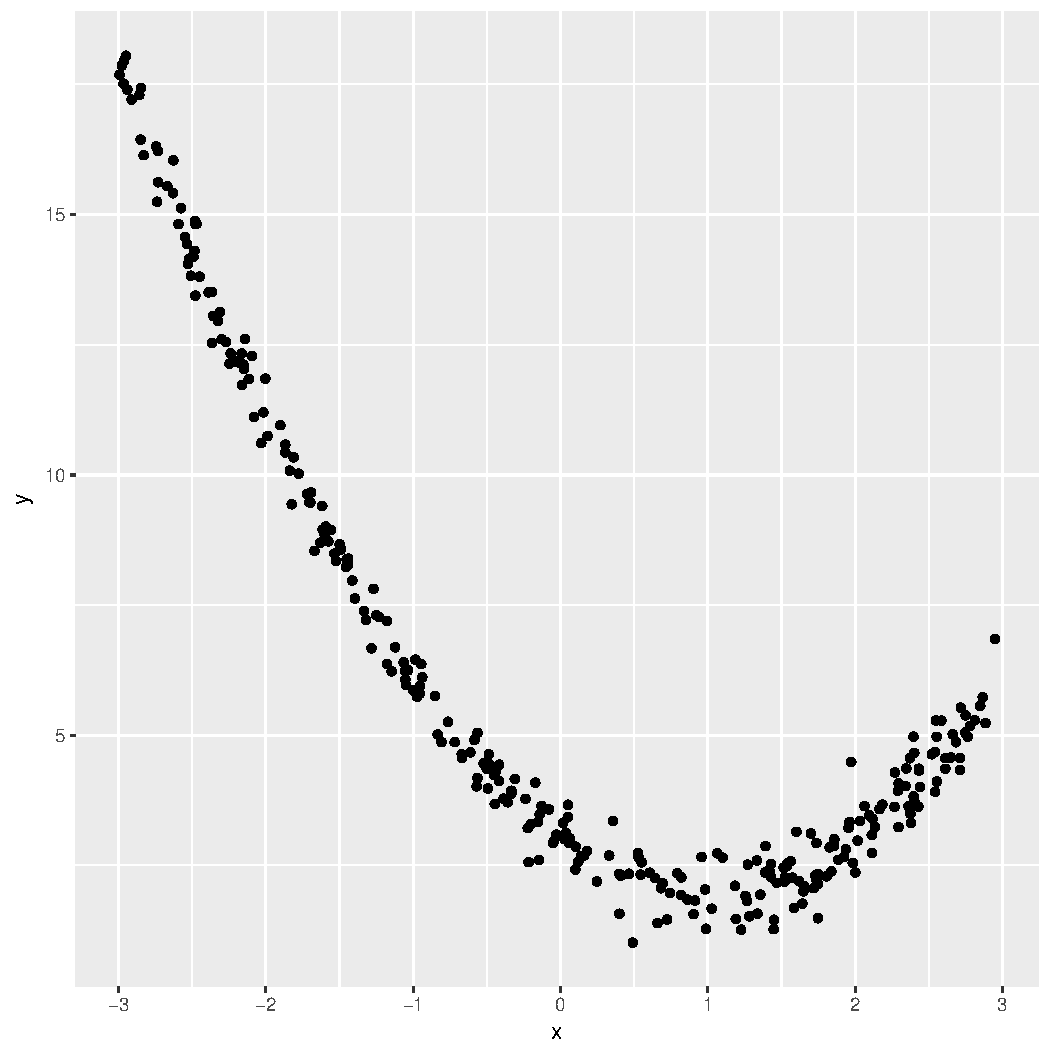
\includegraphics[width=2.5in]{curvy}
\end{figure}

\benum
\subquestionwithpoints{2} If we are now in the statistical learning framework, what subtype of problem are we most likely solving?

\begin{enumerate}[i)]
\item regression to predict $y$
\item binary classification to predict $y$
\item finding $t$ directly
\item finding optimal $n$ and $p$ for $\mathbb{D}$
\item building $\mathcal{A}$ to find $f$ directly
\item estimating $\mathcal{X}$ and $\mathcal{Y}$ using $\mathcal{H}$
\end{enumerate}

\subquestionwithpoints{3} Illustrate the null model $g_0$ as a function of $x$ on the plot above.\spc{-0.5}

\subquestionwithpoints{2} If we are now in the statistical learning framework, what will the final output be of the \emph{learning procedure}?

\begin{enumerate}[i)]
\item $\hat{y}$
\item $\mathcal{A}$
\item $g$
\item $h^*$
\item $h$
\item $f$
\item $z_1, \ldots, z_t$
\end{enumerate}
\pagebreak

\noindent We will be fitting many models to this data. Consider fit \#1 below (the line):

\begin{figure}[htp]
\centering
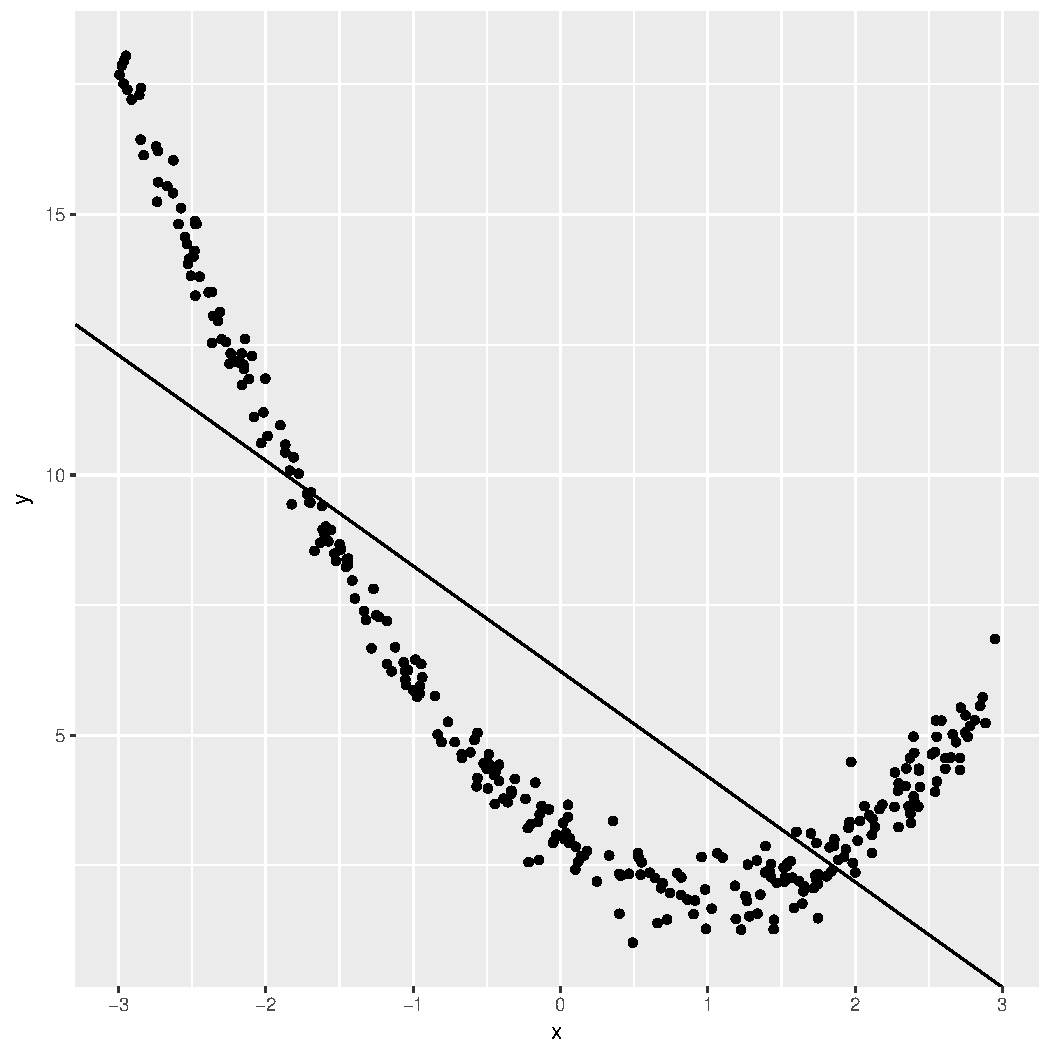
\includegraphics[width=2.5in]{curvyline}
\end{figure}

\subquestionwithpoints{2}  What is the approximate $R^2$ of fit \#1?

\begin{enumerate}[i)]
\item -50\%
\item 0\%
\item 5\%
\item 50\%
\item 95\%
\item 100\%
\end{enumerate}


\subquestionwithpoints{2} If, instead of using $x$ to model $y$, we used $\tilde{x} := \indic{x\geq0}$ to model $y$ and use the same $\mathcal{H}$ (and $\mathcal{A}$) as done in fit \#1, the $R^2$ relative to your answer in (d) would

\begin{enumerate}[i)]
\item decrease
\item remain the same
\item increase
\item not enough information to tell
\end{enumerate}


\subquestionwithpoints{2} In fit \#1, what is most likely the problem?

\begin{enumerate}[i)]
\item misspecification of $\mathcal{H}$
\item $g$ is too far from $t$
\item we are too ignorant of $z_1, \ldots, z_t$ since we only know $x$
\item the $\mathcal{A}$ is not optimizing its cost function correctly
\item $f$ could never be approximated with this $\mathbb{D}$.
\item $h^* \notin \mathcal{H}$
\end{enumerate}
\pagebreak

\subquestionwithpoints{1} In fit \#1, is $g \approx h^*$? Yes/no.\spc{0}

\noindent Consider fit \#2 below:

\begin{figure}[htp]
\centering
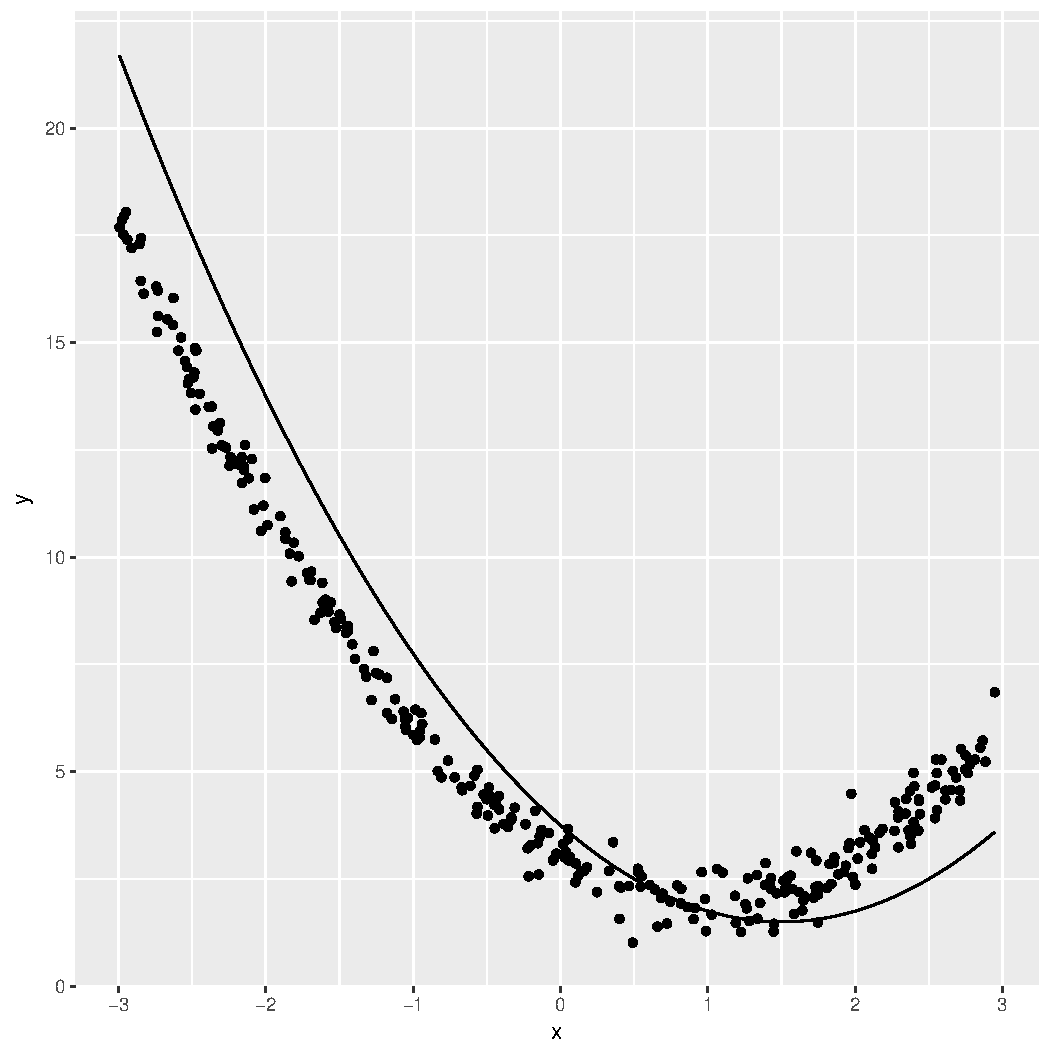
\includegraphics[width=2.5in]{curvybadcurve}
\end{figure}


\subquestionwithpoints{2} In fit \#2, what is most likely the problem?

\begin{enumerate}[i)]
\item misspecification of $\mathcal{H}$
\item $g$ is too far from $t$
\item we are too ignorant of $z_1, \ldots, z_t$ since we only know $x$
\item the $\mathcal{A}$ is not optimizing its cost function correctly
\item $f$ could never be approximated with this $\mathbb{D}$.
\item $h^* \notin \mathcal{H}$
\item non-linear models are illegal and thus this question cannot be answered
\end{enumerate}

\noindent Consider fit \#3 below:

\begin{figure}[htp]
\centering
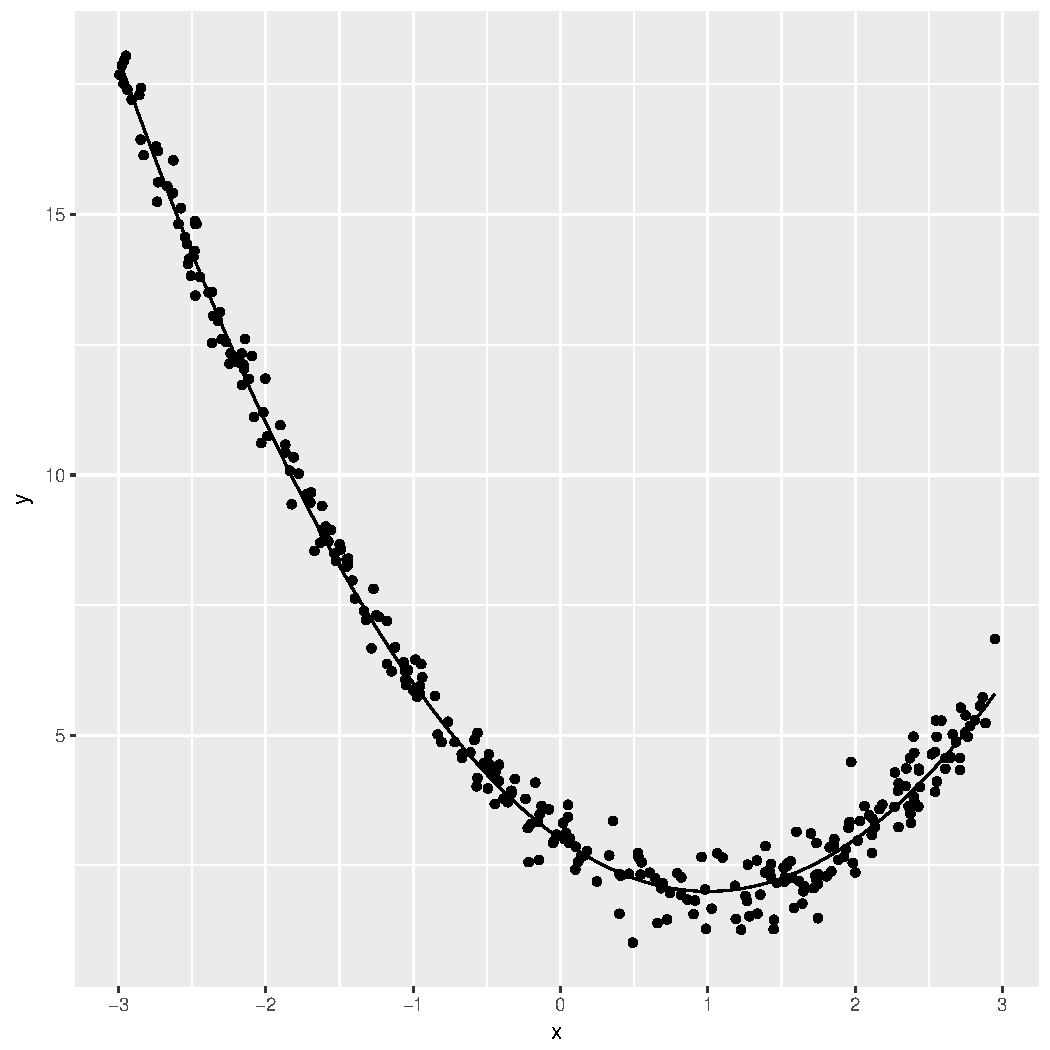
\includegraphics[width=2.5in]{curvygoodcurve}
\end{figure}

\subquestionwithpoints{2} What is the approximate $R^2$ of fit \#3?

\begin{enumerate}[i)]
\item -50\%
\item 0\%
\item 5\%
\item 50\%
\item 95\%
\item 100\%
\item $R^2$ is meaningless if $\mathcal{H} \neq \braces{\w \cdot \x : \w \in \reals^{p + 1}}$.
\end{enumerate}

\subquestionwithpoints{2} What is the approximate RMSE of fit \#3?

\begin{enumerate}[i)]
\item -4
\item 0
\item 0.4
\item 4
\item 40
\item RMSE is always $\bar{y}$
\item RMSE is meaningless if $\mathcal{H} \neq \braces{\w \cdot \x : \w \in \reals^{p + 1}}$.
\end{enumerate}

\subquestionwithpoints{3}  In fit \#3, choose the \emph{likely} largest source of error and indicate a strategy to mitigate it in the future.

\begin{enumerate}[i)]
\item error due to ignorance which can be reduced by \line(1,0){150}
\item misspecification error which can be reduced by \line(1,0){155}
\item estimation error which can be reduced by \line(1,0){182}
\end{enumerate}

\subquestionwithpoints{1}  Regardless of what you think about the fit of the model, consider the following situation. The phenomenon $y$ that we were attempting to predit is \emph{price of a metal per gram in dollars}. And, if the predicted price has to be wrong by more than \$0.25/g for our business to lose money, would this be a \qu{good model}? Yes / no.\spc{-0.5}

\subquestionwithpoints{1}  Regardless of what you think about the fit of the model, consider the following situation. The phenomenon $y$ that we were attempting to predit is \emph{toxicity of a substance}. And, if the predicted toxicity is wrong by even 0.1 then the patient could die, would this be a \qu{good model}? Yes / no.


\subquestionwithpoints{1} Could fits \#1, 2 and 3 be fit with the support vector machine algorithm we discussed in class? Yes/no.\spc{3}

\eenum


\problem This question is another modeling example. Below is a plot of $\mathbb{D}$:

\begin{figure}[htp]
\centering
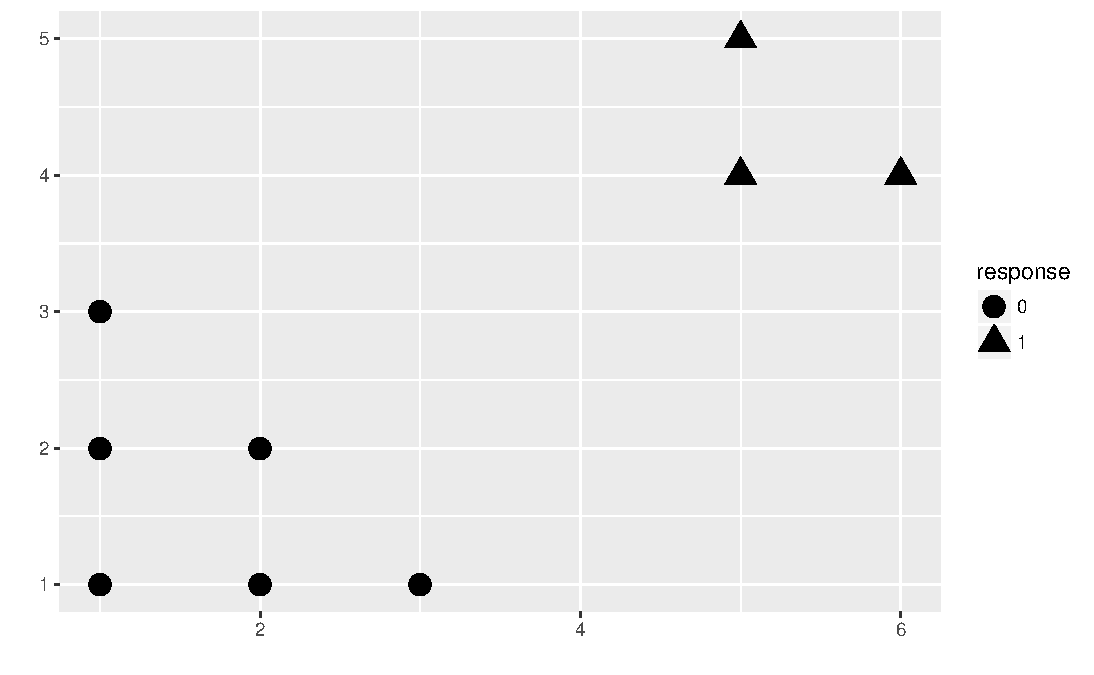
\includegraphics[width=3in]{linsep}
\end{figure}

\benum
\subquestionwithpoints{2} If we are now in the supervised statistical learning framework, what subtype of problem are we most likely solving?

\begin{enumerate}[i)]
\item regression to predict $y$
\item binary classification to predict $y$
\item finding $t$ directly
\item finding optimal $n$ and $p$ for $\mathbb{D}$
\item building $\mathcal{A}$ to find $f$ directly
\item estimating $\mathcal{X}$ and $\mathcal{Y}$ using $\mathcal{H}$
\end{enumerate}

\subquestionwithpoints{2} What is $p$ in this supervised learning problem? What is $n$? Answer both numerically. \spc{0.2}

\subquestionwithpoints{2} What is the null model $g_0$ in this case? \spc{-0.5}

\subquestionwithpoints{3} If you were to use the \emph{perceptron learning algorithm} beginning from random $\w$ locations, draw 3 possible outputs from the algorithm on the plot above. Use dashed lines to illustrate. Also, label the axes. \spc{-0.5}

\subquestionwithpoints{4} For any of the 3 possible outputs from the \emph{perceptron learning algorithm}, provide the function $g$ below explicitly.\spc{0.5}

\subquestionwithpoints{2} If you were to use the \emph{linear support vector machine algorithm} for linearly separable $\mathbb{D}$, draw one possible output from the algorithm on the plot above. Use a solid line to illustrate.\spc{-0.5}


\subquestionwithpoints{1} Of the four models you imagined in parts (c) and (e), which one will give the best performance prediction by and large under general conditions?
\pagebreak

Now consider the same data except with one new data point.


\begin{figure}[htp]
\centering
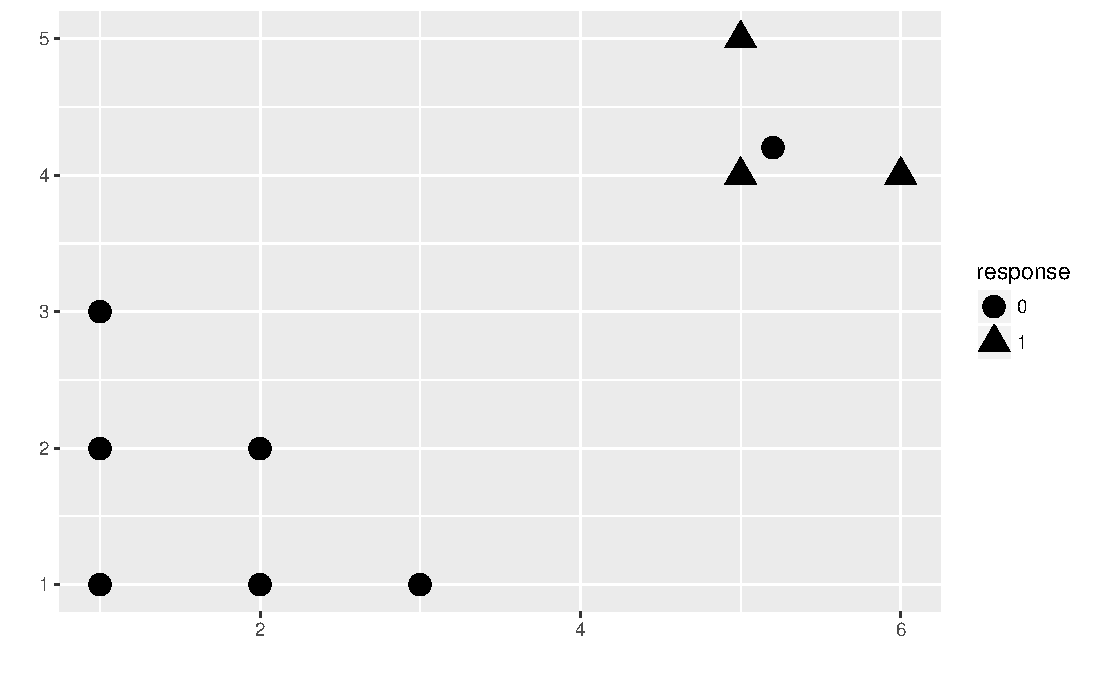
\includegraphics[width=5.7in]{nonlinsep}
\end{figure}

\subquestionwithpoints{3} Consider employing the \emph{linear support vector machine algorithm} for nonlinearly separable $\mathbb{D}$. Let $\lambda = 0$. Draw the most likely output line on the above plot. Use a dashed line to illustrate. Also, label the axes the same as previously. \spc{-0.5}

\subquestionwithpoints{3} Approximate the average hinge loss of the dashed line you drew in the previous question.

\begin{enumerate}[i)]
\item $<0$
\item 0
\item 0.02
\item 0.2
\item 2
\item $>$2
\end{enumerate}

\subquestionwithpoints{3} Consider employing the \emph{linear support vector machine algorithm} for nonlinearly separable $\mathbb{D}$. And let $\lambda > 0$ so that the term that $\lambda$ effects becomes important in the optimization but does not drown out the hinge loss. Draw the most likely output line on the above plot. Use a solid line to illustrate.\spc{-0.5}

\subquestionwithpoints{1} How would the solution you proposed in (i) be fit on a computer?

\begin{enumerate}[I)]
\item There is an analytic solution that is pre-programmed
\item The computer uses numerical optimization which is heuristic
\end{enumerate}

\subquestionwithpoints{2} Consider $\x^* = \bracks{5.4~4.2}$. What is $\hat{y}^*$ if you employ the KNN algorithm where $k=1$? \spc{0}

\subquestionwithpoints{3} Consider $\x^* = \bracks{5.4~4.2}$. What is $\hat{y}^*$ if you employ the KNN algorithm where $k=3$? \spc{0}

\subquestionwithpoints{3} Consider $\x^* = \bracks{5.4~4.2}$. What is $\hat{y}^*$ if you employ the KNN algorithm where $k=10$? \spc{0}
\eenum

\problem Consider a subset of the Boston Housing Data that has been preprocessed. Below is some \texttt{R} code that gives background on the \texttt{boston} data frame which will be referenced throughout this problem. Note that this problem contains some coding exercises. 

\begin{lstlisting}
> dim(boston)
[1] 506   4
> head(boston)
          chas rad  room medv
1 NOT_ON_RIVER   1 6.575 24.0
2 NOT_ON_RIVER   2 6.421 21.6
3 NOT_ON_RIVER   2 7.185 34.7
4 NOT_ON_RIVER   3 6.998 33.4
5 NOT_ON_RIVER   3 7.147 36.2
6 NOT_ON_RIVER   3 6.430 28.7
> summary(boston)
           chas          rad            room           medv      
 NOT_ON_RIVER:471   24     :132   Min.   :3.561   Min.   : 5.00  
 ON_RIVER    : 35   5      :115   1st Qu.:5.886   1st Qu.:17.02  
                    4      :110   Median :6.208   Median :21.20  
                    3      : 38   Mean   :6.285   Mean   :22.53  
                    6      : 26   3rd Qu.:6.623   3rd Qu.:25.00  
                    2      : 24   Max.   :8.780   Max.   :50.00  
                    (Other): 61 
\end{lstlisting}

\benum

\subquestionwithpoints{2} Using the terminology used in class, what type of predictor is \texttt{rad}? \spc{1}

\subquestionwithpoints{2} Using the terminology used in class, what type of predictor is \texttt{room}? \spc{1}


\subquestionwithpoints{2} Write one line of \texttt{R} code below that pulls out the 7th observation as a vector. \spc{1}

\subquestionwithpoints{2} Write one line of \texttt{R} code below that pulls out the first 30 observations. \spc{0.5}

\subquestionwithpoints{3} Write one line of \texttt{R} code below that pulls out all observations where: \texttt{chas} is \qu{\texttt{ON\_RIVER}} or \texttt{medv} is less than 20. \spc{0.5}

\subquestionwithpoints{3} Write one line of \texttt{R} code below that creates a new data frame \texttt{boston\_random} containing the same observations as \texttt{boston} but where the order of the observations is random. \spc{0.5}

\subquestionwithpoints{2} Write one line of \texttt{R} code below that finds the 25\%ile of the variable \texttt{medv}. \spc{0.5}

\subquestionwithpoints{2} What would the following code produce?

\begin{lstlisting}
as.matrix(boston[1 : 2, 3 : 4])
\end{lstlisting}
~\spc{3}

\subquestionwithpoints{1} What would the following code produce?

\begin{lstlisting}
class(as.matrix(boston[, 3: 4])[1, ])
\end{lstlisting}
~\spc{-0.7}


\subquestionwithpoints{1} What would the following code produce?

\begin{lstlisting}
class(as.matrix(boston[, 3: 4])[1, , drop = FALSE])
\end{lstlisting}
~\spc{1}

\eenum

\problem This last problem contains pure coding exercises. 

\benum

\subquestionwithpoints{5} Complete the function below to spec. You don't have to use all the free lines given (in fact, it can be done in one line). You are free to use the \texttt{mean}, \texttt{sd}, \texttt{cov}, \texttt{cor} and other base \texttt{R} functions (but you cannot use \texttt{lm}). \spc{-0.5}

\begin{lstlisting}
#' This function implements the linear least squares regression algorithm
#' popularized by Sir Francis Galton in 1886.
#'
#' @param x		the continuous predictor
#' @param y		the continuous response 	
#' @return 		a list containing a key ``b_0'' whose value is the inter-
#'						cept and a key ``b_1'' whose value is the slope
linear_least_squares_algorithm = function(x, y){












}
\end{lstlisting}

\vspace{0.2cm}
\subquestionwithpoints{2} What does the following code produce? 

\begin{lstlisting}
xs = rep(NA, 5)
xs[3] = -8
xs[5] = 7
tot = 0
for (x in xs){
  if (is.na(x)){
    next
  }
  tot = tot + x
}
tot
\end{lstlisting}


\subquestionwithpoints{1} What does the following code produce? 

\begin{lstlisting}
my_function = function(x, y = 2, z = 3, p = 4, q = 6, r = 0){
  (x + y + z) / (p + q + r)
}
my_function(1)
\end{lstlisting}

\eenum
\pagebreak


\problem Some final theory for extra credit. 

\benum

\subquestionwithpoints{5} [Extra credit] Consider the non-linearly separable SVM algorithm we studied in class. Now, describe an alternative $\mathcal{A}$ which instead of returning a function whose range is only $\braces{0,1}$, returns a function that can estimate $\cprob{Y = 1}{\X = \x}$.  Describe it in English and use diagrams if necessary.\spc{30}

\eenum

\end{document}
